\documentclass{article}
\usepackage{macro}
\begin{document}

Policy gradient methods attempt to update the parameter of the policy
$\pi_{\theta}$ in the way that maximizes the expected return
\[
    J(\theta) \definedas \int_{\A \times \S}\mu(s)
    \pi_{\theta}(a|s)A(a, s) dads
\]
This is equivalent to maximize likehood of actions $a$ (conditioned over
$s$) according to its advantage. 

But this is not an optimization problem, as we do not want to make 
good actions "too likely". This is because state visitation distribution
depends on the policy itself, big change in policy creates big change
of state visitation, so overly optimized action likelihood conditioned
on previous state visitation would underfit for the state visitation 
under updated policy (one instance of bias variance trade off).
This is a distinctive difference to the supervised learning, in SL we 
do want to solve maximum likelihood estimator as optimization problem,
because the distribution of input data stays unchanged throughout the 
training.

TRPO attempts to treat policy gradient methods as an optimization 
problem by constraining the policy update to a trust region
\begin{align*}
    & \theta_{k+1} = \argmax_{\theta} \E_{(a,s)\sim \pi_{\theta_k}} 
        (\frac{\pi_{\theta}(a|s)}{\pi_{\theta_k}(a|s)} A^{\theta_k}(a, s) \\
    & D_{KL}(\theta || \theta_k) < \delta
\end{align*}

within the trust region, we assume the state visitation distribution
stays constant, so that policy gradient RL becomes SL locally inside
the trust region. 

We needs to compute the Hessian of the parametric policy in order to 
compute the step size of the policy update (maximum update and stay in 
the trust region). Compute Hessian directly involves $O(N^2)$ time and
space ($N$ number of parameters). We can avoid computing the Hessian 
through conjugate gradient methods. This reduces the problem to $C O(N)$
where $C$ is the number of conjugate gradient iterations. Take away is
TRPO can be computationally expensive.


PPO attepmts to solve the same problem as TRPO: get the biggest step
size for policy update without breaking the policy. 

PPO only involves first-order optimization. According to the published
results, the performance of PPO is just as good as TRPO. 

Two variants of PPO

\textbf{PPO-Clip} does not use KL-divergence to make the new policy 
close to the old one. It clips the surrgate gain (it clips the 
$\frac{\pi(a|s)}{\pi_{\text{old}}(a|s)}$ term to $(1 - \epsilon, 
1 + \epsilon)$ range to make sure the policy update is not too big. 
This behaves like trust region method.

\textbf{PPO-Penalty} solves the KL-contrained update like TRPO. It 
penalizes the KL-divergence in the objective instead of making it a 
hard constraint. The penalty coefficiently is adjusted automatically 
throughout the training. 


\section{PPO-Clip}
PPO-Clip updates policies via
\[
\theta_{k+1} = \argmax_{\theta}\E_{s, a\sim \pi_{\theta_k}}
[L(s, a, \theta_k, \theta)]
\]
where 
\[
L(s, a, \theta_k, \theta) = \min(
\frac{\pi_{\theta}(a|s)}{\pi_k(a|s)}A^{\pi_k}(s, a), \text{clip}(
\frac{\pi_{\theta}(a|s)}{\pi_k(a|s)}, 1-\epsilon, 1 + \epsilon)
A^{\pi_k}(s, a))
\]

Interpretation:
$\text{clip}(\frac{\pi_{\theta}(a|s)}{\pi_{\theta_k}(a|s)}, 
1-\epsilon, 1 + \epsilon)$ makes 
$\pi_{\theta}(a|s) \in [(1-\epsilon)\pi_{\theta_k}, (1+\epsilon)
\pi_{\theta_k}]$

Suppose $A^{\pi_k}(a|s) <0$, you want to make $a$ less likely. The 
update objectively says $\pi_{k+1}(a|s) \geq (1-\epsilon)\pi_k(a|s)$;
conversely, if $A^{\pi_k}(a|s)$ is positive, you want to make $a$
more likely in your next policy iteration, the objective says
$\pi_{k+1}(a|s) \leq (1 + \epsilon)\pi_k(a|s)$.

The objective says the new policy can be at most $\epsilon$ "units" 
away from the old policy. This is some sort of trust-region 
optimization, $\epsilon$ defines the size ofthe trust region.  

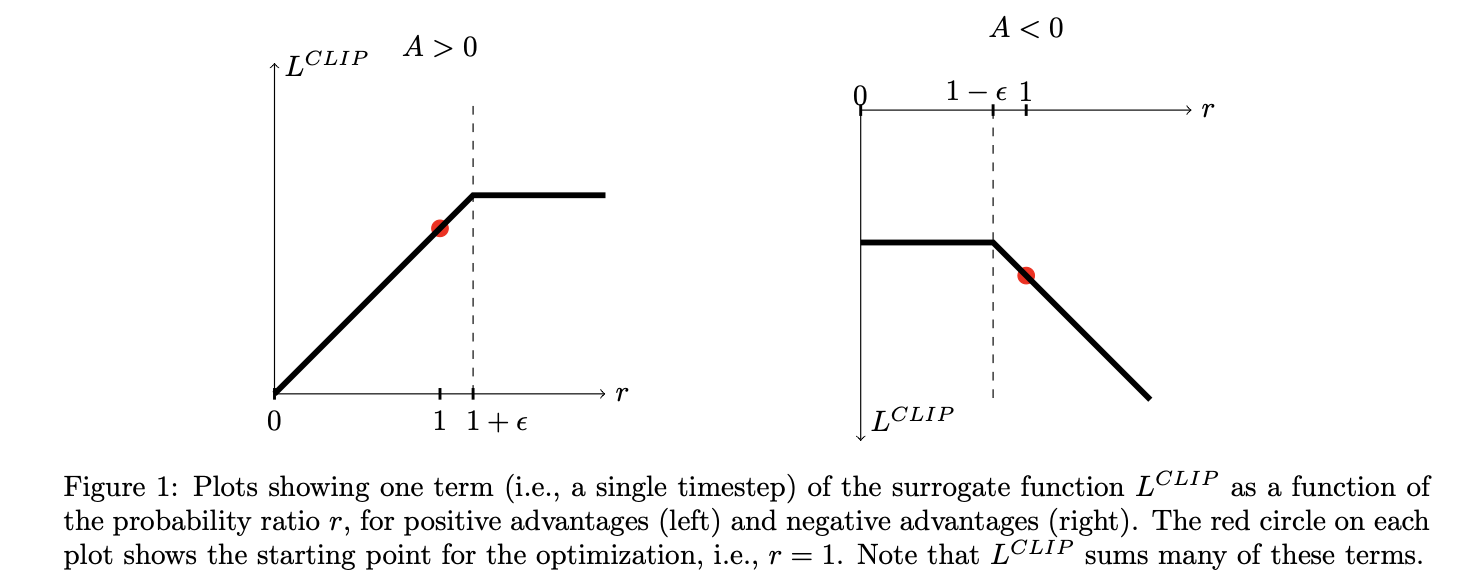
\includegraphics[width=12cm]{ppo_clip}

\begin{algorithm}[H]
\caption{PPO-clip}
\label{alg1}
\end{algorithm}
Let $g(\theta, A^{\pi_k}(s,a)) = \text{clip}(
\frac{\pi_{\theta}(a|s)}{\pi_k(a|s)}, 1-\epsilon, 1 + \epsilon)
A^{\pi_k}(s, a))$

\begin{algorithmic}[1]
\STATE Input: initial policy $\theta_0$, initial value function $\phi_0$
\FOR{$k=0,1,\cdots,$}
\STATE Collect a set of trajectories $D_k = \{\tau_i\}$ by running policy
$\pi_k$ in the env
\STATE Compute rewards-to-go $\hat R_t$ ($G$)
\STATE Compute advantage estimate $\hat A_t$ based on the current
value function $\phi_k$
\STATE Update the policy by maximizing the PPO-Clip objective
\[
\theta_{k+1} = \argmax_{\theta} \frac{1}{|D_k|T}
\sum_{\tau \in D_k}\sum_{t=0}^T \min(
\frac{\pi_{\theta}(a_t | s_t)}{\pi_{\theta_k}(a_t|s_t)}
A^{\pi_{\theta_k}}(s_t, a_t), g(\epsilon, A^{\pi_k}(s_t, a_t)))
\]
typically via Stochastic ascend with Adam

\STATE Fit value function by regression on mean-squared error:
\[
\phi_{k+1} = \argmin_{\phi}\frac{1}{|D_k|T}
\sum_{\tau \in D_k}\sum_{t=0}^T(V_{\phi}(s_t) - \hat R_t)^2
\]
typically via some gradient descent algorithm. 
\ENDFOR
\end{algorithmic}

\section{PPO-Penalty}
Another approach to do policy iteration and regulate the risk of breaking
the policy is to treat the KL divergence (with the old policy) as a 
penalty in the loss objective. In supervised deep learning, we can the
analogous idea of prevent the network from overfitting the data by L2 
weight decay. 

The objective we want to maximize is 

\[
L^{KLPEN}(\theta) = \E_{t}[
\frac{\thetapi(a_t|s_t)}{\oldpi(a_t | s_t)}\hat A_t
- \beta \KL[\oldpi(\cdot | s_t), \thetapi(\cdot|s_t)]
]
\]

$\beta$ is an \emph{adaptive} parameter determined by the 
\[
d = \E_t[\KL[\oldpi(\cdot | s_t), \thetapi(\cdot | s_t)]]
\]

- If $d < d_{targ}/1.5$, $\beta \leftarrow \beta/2$

- If $d > d_{targ}/1.5$, $\beta \leftarrow \beta * 2$



\begin{algorithm}[H]
\caption{PPO-KL}
\label{alg2}
\end{algorithm}

\begin{algorithmic}[2]
\STATE Input: initial policy $\theta_0$, initial value function $\phi_0$,
a KL penalty coefficient $\beta$, a trust region size $d_{targ}$
\FOR{$k=0,1,\cdots,$}
\STATE Collect a set of trajectories $D_k = \{\tau_i\}$ by running policy
$\pi_k$ in the env
\STATE Compute rewards-to-go $\hat R_t$ ($G$)
\STATE Compute advantage estimate $\hat A_t$ based on the current
value function $\phi_k$
\STATE Determine the KL penalty coefficient by
\[
d = \E_t[\KL[\oldpi(\cdot | s_t), \thetapi(\cdot | s_t)]]
\]

\IF {$d < d_{targ} / 1.5$}
    \STATE $\beta \leftarrow  \beta / 2$
\ELSIF {$d > d_{targ} * 1.5$}
    \STATE $\beta \leftarrow \beta *2 $
\ENDIF

\STATE Update the policy by maximizing the PPO-KL objective
\[
L^{KLPEN}(\theta) = \E_{t}[
\frac{\thetapi(a_t|s_t)}{\oldpi(a_t | s_t)}\hat A_t
- \beta \KL[\oldpi(\cdot | s_t), \thetapi(\cdot|s_t)]
]
\]

typically via Stochastic ascend with Adam

\STATE Fit value function by regression on mean-squared error:
\[
\phi_{k+1} = \argmin_{\phi}\frac{1}{|D_k|T}
\sum_{\tau \in D_k}\sum_{t=0}^T(V_{\phi}(s_t) - \hat R_t)^2
\]
typically via some gradient descent algorithm. 
\ENDFOR
\end{algorithmic}


How to get this algorithm into code?

1. Importance sampling interpretation of the policy loss allows us to use experiences 
from an old policy to update the current policy. The trajectory sampled from
$\theta_k$ can be used by the algorithm to update $\pi$ \textbf{a couple of times}. 
Each time of the update, we can compute 
$\frac{\pi_{\theta}(a|s)}{\pi_{\theta_k}(a|s)}A^{\pi_k}(a, s)$ and clip it to 
$[(1-\epsilon)A, (1 + \epsilon)A]$ and compute the gradient of the loss with 
respect to the parameters of $\pi_{\theta}$. This is somehow making the PPO a 
slightly-off-policy algorithm.

2. It might also be a good idea to clip the loss of the value function. 

3. How do deep learning framework implement loss clipping? It is a node 
in a computation graph and it is not a differentiable operation? Same 
question goes to absolute value? I think they probably use some bump
function that decreases sharply near the boundary points (clipping range).
Same thing with absolute value, they probably have some way to smooth
out the function at 0.

4. Good implementation of PPO uses parallel env to sample trajectory 
from many envs (see A2C). 

\end{document}
